\documentclass{ib-assignment}


\usepackage[english]{babel}
\usepackage[utf8]{inputenc}
\usepackage{amsmath}
\usepackage{relsize}
\usepackage{graphicx}
\usepackage{tikz}
\usepackage{amsthm}
\usetikzlibrary{decorations.pathreplacing}
\usepackage[colorinlistoftodos]{todonotes}


%%%%%%%%%%%%%%%%%%%%%
% INFO
%%%%%%%%%%%%%%%%%%%%%%
\title{Functional Neural Networks}

\author{William Guss}
\candidatenum{000345-0022}
\subtitle{Approximated by Weierstrass Polynomials}
\subject{Mathematics}
\advisor{Nathaniel Nelson}
\wordcount{3900}
\setabcount{100}
\updateheaders
\date{May 2015}
    \def\layersep{2cm}

%%%%%%%%%%%%%%%%%%
%BIBLIOGRAPHY
%%%%%%%%%%%%%%%%%%
\usepackage{csquotes}
\usepackage[style=ieee, backend=biber]{biblatex}
\addbibresource{FNN.bib}

%%%%%%%%%%%%%%%
% MATH
%%%%%%%%%%%%%%%
\newtheorem{definition}{Definition}[section]
\newtheorem{lemma}{Lemma}
\newtheorem{theorem}{Theorem}
\newtheorem{corollary}{Corollary}
\newcommand{\Sum}{\mathlarger{\mathlarger{\sum}}}

\begin{document}
\maketitle

\begin{abstract}
\normalsize
In this paper we consider the traditional model of feed-forward neural networks proposed in (McCulloch and Pitts, 1949), and using intuitions developed in (Neal, 1994) we propose a method generalizing discrete neural networks as follows.
In the standardized case, neural mappings $\mathcal{N}: \mathbb{R}^n \to [0,1]^m$ have little meaning when $n \to \infty$. Thus we consider a new construction $\mathcal{F}: \mathcal{X} \to \mathcal{Y}$ where the domain and co-domain of $\mathcal{N}$ become infinite dimensional Hilbert spaces, namely the set of quadratically Lebesgue integrable functions $L^2$ over a real interval $E$ and $[0,1]$ respectively.
 The derivation of this construction is intuitively similar to that of Lebesgue integration; that is, $\sum_i \sigma_i w_{ij} \to \int_{E\subset\mathbb{R}}\sigma(i)w(i,j)\ d\mu(s)$. 

After establishing a proper family of "functional neural networks" $\mathcal{F}$, we show that $\mathcal{N}$ are a specific class of functional neural networks under specific constraints. More specifically in our first lemma, we prove that $\mathcal{F} \equiv \mathcal{N}$ for piecewise constant weight functions $w(i,j)$. Having done so, we then attempt to find an analogue to Cybenko's theorem of universal approximation for neural networks. Firstly, we prove as a corollary of the Weierstrass approximation theorem, that $w(i,j)$ can approximate with arbitrary precision a function satisfying $\left\|\mathcal{F}\xi - f(\xi)\right\|_\infty \to 0$ for arbitrary $f:E\to[0,1]$. As a byproduct of the proof, we also establish a closed-form definition for the satisfying $w(i,j)$ and thereby through our first lemma provide novel insight into the actual form of the weight matrix $[w_{ij}]$ for trained $\mathcal{N}$. Finally we propose a universal approximation theorem for functional neural networks; that is, we show through the Riesz Representation Theorem that $\mathcal{F}$ approximates any bounded linear operator on $\mathcal{X}$.

In conclusion, we create a practical analogue of the error-backpropagation algorithm, and implement functional neural networks using Simpson’s rule. We suggest that functional neural networks represent an interesting opportunity for the implementation of machine learning systems modeling functional transformation.
\abcount
\end{abstract}

\newpage
\tableofcontents
\newpage
\section{Introduction}
Machine learning is a highly interdisciplinary field which deals with the development of algorithms that can predict and classify novelties based on a set of prior “intuitions” \cite{mlsurvey}. The field itself employs research from biology, computer science, numerical analysis, and statisitics. In recent years applications of machine learning can be seen holistically throughout our society in web services like Google, Facebook, and Amazon to name a few. Seeing as there is incentive from both private industry and academia, machine learning is ever expanding and developing as an integral field of mathematical and scientific inquiry.  


One of the most biologically inspired set of algorithms developed in the field is the artificial neural network (ANN). Although there are numerous mathematical interpretations of neural networks, we will primarily focus on the expansion of one such interpretation, feed-forward neural networks. In order to understand this specific interpretation, some biological foresight is required.
\subsection{Biological Neurons}
A single neuron consists largely of the cell body or soma, the dendrites, and the axon. Mathematically we wish to examine the process of neural activation, namely the events which lead to the excitation of the axon. Consider a neuron whose anterior neurons (those which are connected dendritically) are activated; that is, the neuron is receiving input along all of its dendrites. These electrical inputs propagate through the dendrites and then become integrated on the Soma as electrical membrane potential \cite{griffith}. The soma then acts as the primary computational unit and activates the axon when a threshold of input activity is reached. More specifically, when a memberane potential of about -60 mV is reached on the soma, the hillock zone, or axon hillock, activates the axon by applying proteins to an ion channel which creates action potential along the axon \cite{bioneuron}.
\subsection{Artificial Neurons}
\begin{figure}
\centering
\includegraphics{neuron}
\caption{A biological neuron \cite{neuralimage}.}
\end{figure}
	With this in mind it is now possible to construct a mathematical model of an artificial neuron. Let \( A_j, P_j\) be the set of anterior and posterior neurons of a neuron, \(j\). Then, the cell membrane naturally becomes a linear combination of the dendritic potentials.
   \begin{definition}
   We say that \(\mathrm{net}_j\) is the net electric potential over the membrane, if for a natural neural resting potential \(\beta\), 
\[ \textrm{net}_j = \Sum_{i \in A_j}{w_{ij}\sigma_i} + \beta \]where \(w_{ij}\) is the dendritic connection “strength” from the \(i\)\textsuperscript{th} anterior neuron to \(j\), \(\sigma_i\) is the action potential being propagated from the \(i\)\textsuperscript{th} anterior neuron. 
   \end{definition}
   
Furthermore, the thresholding of the hillock zone is given by some real valued sigmoidal function \(g\) bijective and differentiable over \(\mathbb{R}\). 
\begin{definition}
We call \(\sigma_j\) the action potential  of a neuron \(j\) if  
\[\sigma_j = g\left(\mathrm{net}_j\right)\]
for some continuous real valued, monotonically increasing function \(g\).
\end{definition}
This model of the artifical neuron follows from the work that Pitt and McCulloch did in representing neural activity as logical thresholding elements  \cite{mcculloch}.
%\todo{improve}

\subsection{Feed-Forward Artificial Neural Networks}
	Now we have sufficient mathematical basis to define the feed-forward artificial neural network. The concept of a feed-forward ANN is biologically motivated by the functional organization of the visual cortex. It is appropriate to divide the structure of the visual cortex into layers which are denoted V1, V2, V3, and so on. The layers are organized such that a given layer is directly adjacent to and exhibiting full connectedness to the subsequent layer, an example being V1 to V2, V2 to V3, and subsequently for all of the primary layers of the visual cortex. From a functional point of view these layers store levels of visual abstraction like lines and shapes on the lower layers to faces and abstract visual concepts on the highest layers\cite{visualcortex}.

\begin{figure}
\centering
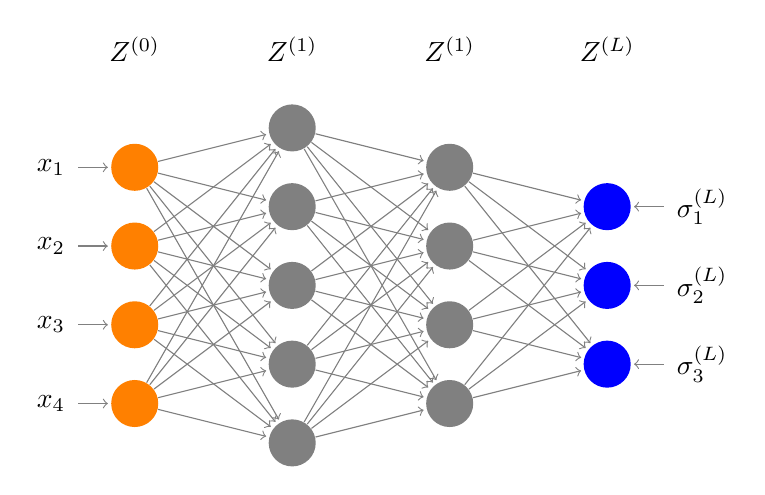
\begin{tikzpicture}[shorten >=1pt,->,draw=black!50, node distance=\layersep]
    \tikzstyle{every pin edge}=[<-,shorten <=1pt]
    \tikzstyle{neuron}=[circle,fill=black!25,minimum size=17pt,inner sep=0pt]
    \tikzstyle{input neuron}=[neuron, fill=orange];
    \tikzstyle{output neuron}=[neuron, fill=blue!100];
    \tikzstyle{hidden neuron}=[neuron, fill=black!50];
    \tikzstyle{annot} = [text width=4em, text centered]

    % Draw the input layer nodes
    \foreach \name / \y in {1,...,4}
    % This is the same as writing \foreach \name / \y in {1/1,2/2,3/3,4/4}
        \node[input neuron, pin=left: \(x_\y\)] (I-\name) at (0,-\y) {};

    % Draw the hidden layer nodes
    \foreach \name / \y in {1,...,5}
        \path[yshift=0.5cm]
            node[hidden neuron] (H1-\name) at (\layersep,-\y cm) {};
            
     \foreach \name / \y in {1,...,4}
        \path[yshift=0.5cm]
            node[hidden neuron] (H2-\name) at (2*\layersep,-0.5cm -\y cm) {};

    % Draw the hidden layer nodes
    \foreach \name / \y in {1,...,3}
        \path[yshift=0.5cm]
            node[output neuron, pin=right:\(\sigma_{\name}^{(L)}\)] (O-\name) at (3*\layersep,-1cm -\y cm) {};


    % Connect every node in the input layer with every node in the
    % hidden layer.
    \foreach \source in {1,...,4}
        \foreach \dest in {1,...,5}
            \path (I-\source) edge (H1-\dest);

    % Connect every node in the hidden layer with the output layer
    
        \foreach \source in {1,...,5}
    	\foreach \dest in {1,...,4}
        \path (H1-\source) edge (H2-\dest);
    \foreach \source in {1,...,4}
    	\foreach \dest in {1,...,3}
        \path (H2-\source) edge (O-\dest);

    % Annotate the layers
    \node[annot,above of=H1-1, node distance=1cm] (hl) {\(Z^{(1)}\)};
    \node[annot,left of=hl] {\(Z^{(0)}\)};
    \node[annot,right of=hl] {\(Z^{(1)}\)};
    \node[annot,above of=O-1, node distance=2cm] (ol) {\(Z^{(L)}\)};
\end{tikzpicture}
  \caption[An example of a feed-forward ANN]{An example of a feed-forward ANN,  \(\mathcal{N}\) with four layers.}
\end{figure}
The goal then of describing a feed-forward artificial neural network is to model this representation of increasing abstraction whilst maintaing adjacency and full topological connectedness. Thus we construct a set of neural layers with cardinality \(L+1\), and connections as depicted in Figure 2.
    
    \begin{definition}
    
    We say $\mathcal{N}$ is a feed-forward neural network if for an input vector $\pmb{x}$,
	\[
    	\begin{aligned}
        \mathcal{N}:\ & \sigma_j^{(l+1)} &= g\left(\Sum_{i \in Z^{(l)}}w_{ij}^{(l)}\sigma_i^{(l)} + \beta^{(l)}\right) \\ & \sigma_j^{(1)} &= g\left(\Sum_{i \in Z^{(0)}}w_{ij}^{(0)}x_i + \beta^{(0)} \right)
        \end{aligned}
    \]
    where $1\leq l \leq L-1$. 
    \end{definition}
    
    For mathematical convenience let us denote \( \sigma_j^{(l)}\) as the output of the \(j\)\textsuperscript{th} neuron on layer \(l\). In this construction we prefer three different types of neurons, the input neuron, the hidden neuron, and the output neuron. In the case of the input neuron, there is no sigmoidal activation function, and instead we assign each \( \sigma_j^{(0)}\) to a real value which is then weighted by the dendritic input strength of each anterior neuron. Moreover an input neuron only exists on the \(0\)\textsuperscript{th} layer. In the case of each hidden layer we adopt the model described for the standard neuron as aforementioned where our sigmoid activation function \(g = \tanh(\mathrm{net})\)  is the hyperbolic tangent.%\todo{Why?}
Finally, the output layer usually have a linear sigmoid activation as to achieve output scaling beyond \([1,-1]\) in the previous layers. Once again the output layer can only exist on the layer \(L\).  
    %\todo{Personal pronouns} 

\subsection{Error Backpropagation}
   With the  functional organization of the network complete, we now need to develop the notion of learning. For the purposes of this paper we will describe a gradient descent method for learning called error-backpropagation. In the mathematical model we find conveniently that the degrees of freedom are then the dendritic weights between any two neurons. Thus these weights must be optimized against some desired output. This leads to the following multi-dimensional error function.
   \begin{definition} We call E the error function of a neural network $\mathcal{N}$, if for an input vector \(\pmb{x}\)
\[ E\left(w_{00}^{(0)}, w_{01}^{(0)}, \dots ,w_{ij}^{(L)}\right) = \frac12\Sum_{i \in Z^{(L)}}{\left(\sigma_i^{(L)}-\delta_i\right)^2}\]where \(\pmb{\delta}\) is some desired output vector corresponding to \(\pmb{x}\). 
\end{definition}

Then the goal is to optimize this error function such that a reasonable local minimum is found. We then choose to modify each weight in the direction of greatest decrease for the error function. 
\begin{definition}
We call \(\pmb{\nabla}E\) the gradient of \(E\) if 
\[\pmb{\nabla}E = \left(\frac{\partial E}{\partial w_{00}^{(0)}}, 
\frac{\partial E}{\partial w_{01}^{(0)}},\dots,
\frac{\partial E}{\partial w_{ij}^{(L)}}\right)\]
for all weights, \(w_{ij}^{(l)}\), in feed-forward ANN \(\mathcal{N}\).
\end{definition}
\begin{figure}
\centering
 \includegraphics[width=4in]{gradient_descent}
 \caption{Gradient descent on \(E\left(\pmb{x}, \pmb{\delta}\right)\) with descent path shown in blue.}
\end{figure}
Conveniently the gradient of a function describes a vector whose direction is the greatest increase of a function. Thus to optimize our weights so that the lowest error is achieved, we update the weights as follows: \(\pmb{w}(t+1) = \pmb{w}(t)-\alpha \pmb{\nabla}E\) where alpha is some learning rate, a process which is depicted in Figure 3 \cite{rumelhart1988learning}.


The calculation of each \(\frac{\partial E}{\partial w_{ij}^{(L)}}\) is non-trivial given that each weight influences the error function in multiple ways.  To find the contribution of a single weight, recall that every single neuron is connected to all neurons in the anterior and posterior layers. So, a single weight will influence not only its posterior neuron’s sigmoidal output but also that of every neuron for any path from the posterior neuron to the set of output neurons. Thus, the multiplicity of contribution via different neural routes follows directly from the multidimensional chain-rule. Recall the differential operator \(D_g f=\frac{\partial f}{\partial x}\),
\begin{equation*}
	\begin{aligned}
    \frac{\partial E}{\partial w_{ij}^{(l)}} &= D_{\sigma_0^{(L)}}\cdot D_{\mathrm{net}} \sigma_0^{(L)} \cdot D_{\sigma_0^{(L-1)}}\mathrm{net}\cdot \  \cdots \  \cdot  D_{\mathrm{net}} \sigma_j^{(l+1)} \cdot D_{w_{ij}^{(l)}}\mathrm{net} \\
    &+\  D_{\sigma_1^{(L)}}\cdot D_{\mathrm{net}} \sigma_1^{(L)} \cdot D_{\sigma_0^{(L-1)}}\mathrm{net}\cdot\  \cdots \  \cdot  D_{\mathrm{net}} \sigma_j^{(l+1)} \cdot D_{w_{ij}^{(l)}}\mathrm{net} \\
    &\ \vdots\\
    &+\  D_{\sigma_n^{(L)}}\cdot D_{\mathrm{net}} \sigma_n^{(L)} \cdot D_{\sigma_0^{(L-1)}}\mathrm{net}\cdot \  \cdots \  \cdot  D_{\mathrm{net}} \sigma_j^{(l+1)} \cdot D_{w_{ij}^{(l)}}\mathrm{net} \\
        &+\  D_{\sigma_0^{(L)}}\cdot D_{\mathrm{net}} \sigma_0^{(L)} \cdot D_{\sigma_1^{(L-1)}}\mathrm{net}\cdot \  \cdots \  \cdot  D_{\mathrm{net}} \sigma_j^{(l+1)} \cdot D_{w_{ij}^{(l)}}\mathrm{net} \\
            &\ \vdots\\
        &+\  D_{\sigma_n^{(L)}}\cdot D_{\mathrm{net}} \sigma_n^{(L)} \cdot D_{\sigma_1^{(L-1)}}\mathrm{net}\cdot \ \cdots \  \cdot  D_{\mathrm{net}} \sigma_j^{(l+1)} \cdot D_{w_{ij}^{(l)}}\mathrm{net} \\
                &\ \vdots \\
                        &+\  D_{\sigma_n^{(L)}}\cdot D_{\mathrm{net}} \sigma_n^{(L)} \cdot D_{\sigma_m^{(L-1)}}\mathrm{net}\cdot \ \cdots \ \cdot  D_{\mathrm{net}} \sigma_j^{(l+1)} \cdot D_{w_{ij}^{(l)}}\mathrm{net} \\
                        &= \Sum_{a_1}^{Z^{(L)}}\ \Sum_{a_2}^{Z^{(L-1)}} \cdots \Sum_{a_m}^{Z^{(l+2)}} \frac{\partial E}{\partial \sigma_{a_1}^{(L)}}\frac{\partial \sigma_{a_1}^{(L)}}{\partial \mathrm{net}} \frac{\partial \mathrm{net}}{\partial \sigma_{a_2}^{(L-1)}} \ \cdots\ \frac{\partial \sigma_{a_m}^{(l+2)}}{\partial \mathrm{net}}\frac{\partial \mathrm{net}}{\partial \sigma_{j}^{(l+1)}}  \frac{\partial \sigma_{j}^{(l+1)}}{\partial \mathrm{net}} \frac{\partial \mathrm{net}}{\partial w_{ij}^{(l)}}
	\end{aligned}
\end{equation*} %\todo{analysis}
%\todo{new sect}
This construction is of serious mathematical interest as feed-forward neural networks have been shown to be universal approximators; that is, they can approximate any \(f:A\to B\), where \(A,B \in \mathbb{R}^m\) are vector spaces.  In this paper we will generalize the notion of the universal approximation for arbitrary vector space mappings to arbitrary approximation of any\(f:L^1 (\mathbb{R}^n)\to C^\infty(\mathbb{R}^n)\) by examining the structure of feed-forward ANNs as the number of nodes for each layer becomes uncountably bounded in\(\mathbb{R}^n\). Such a generalization requires that a continuum of neural components be made, and that a continuous weight tensor or hypersurface must exist in order to maintain the topological connectedness as prescribed by the discrete model. 
%\todo{incomplete}




\newpage
\section{Functional Neural Networks}
%\todo{badintro} 
Although neural networks have proven an extremely effective mechanism of machine learning \cite{mlsurvey}, theoretically they remain a black-box model.  In answer to this problem Neal examined the notion of infinite hidden nodes with a network proving that such a construction becomes a Gaussian kernel \cite{neal}. Then, Roux and Bengio described a model for affine neural networks with continuous hidden layers in alignment with Neal's reasearch. These authors showed effectively the viability of a "continuous" neural network, but left many similar constructions unexplored. It is the subject of this paper to generalize the construction of a feed-forward ANN which maps uncountably infinite vector spaces, and then to demonstrate the practical implementations of algorithms such as error backpropagation in this generalized form.
\subsection{The Core Idea}
Suppose that we wish to map one functional space to another with a neural network. Consider the standard model of an ANN as the number of nueral nodes for every layer becomes uncountable. The index for each node then becomes real-balue, along with the weight and input vectors %\todo{misleading}
. Let us denote \(\xi: \mathbb{R}^n\to\mathbb{R}\) as some arbitrary input function for the neural network. Likewise consider a real-valued weight function, \(w^{(l)}: \mathbb{R}^{2n}\to\mathbb{R}\), for a later $l$ which is composed of two indexing variables $i,j \in \mathbb{R}^n$. Finally as the number of neural nodes becomes uncountable we define a real-valued bound for any given layer $R^{(l)} \supset Z^{(l)}$.  As the indices become real valued, examination of the sigmoidal sum seen in definition 1.1 leads us to the following derivation
\begin{equation*}
\begin{aligned}
	\sigma^{(1)}(j) &= \lim_{\Delta i \to 0}g\left(\Sum_{i\in R^{(0)}} \xi(i) w^{(0)}(i,j)\ \Delta i + \beta\right) \\
    &= g\left(\int_{R^{(0)}} \xi(i) w^{(0)}(i,j)\ di + \beta\right)
\end{aligned}
\end{equation*}
Repeating the process inductively for all layers in a neural network, leads to a recurrance relation for this construction. 
\begin{definition}
We call $\mathcal{F}$ a functional neural network if,
\begin{equation*}
    	  \begin{alignedat}{2}
        \mathcal{F}:\ &\sigma^{(l+1)}(j) & &=  g\left(\int_{R^{(l)}} \sigma^{(l)}(i) w^{(l)}(i,j)\ di + \beta\right)  \\
        &\sigma^{(0)}(j) & &= \xi(j) 
        \end{alignedat}
\end{equation*}
\end{definition}
To demonstrate the accuracy of this generalization, let us propose the following lemma which is near that of Roux and Bengio.
\begin{theorem} Suppose $\mathcal{F}$ is a functional neural network with a set of piecewise constant weight functions $W = \left\{w^{(0)}, w^{(1)}, \dots, w^{(L-1)}\right\}$ each with constituent pieces of length one. Then given the input function $\xi(i) = x_n, n = \max\left\{m\in \mathbb{Z}\ |\ m\leq i\right\}$ for some input vector $\pmb{x}$, $\mathcal{F}$ is discretized; that is assuming $i,j \in \mathbb{R}$ and $Z^{(l)} = R^{(l)}\ \cap \mathbb{Z}$ then for $0 \leq l \leq L-1$ we have that
$$\mathcal{F}(\xi)\equiv \mathcal{N}(\pmb{x})$$
\end{theorem}
\begin{proof}
Let $P(l)$ be the proposition that $\sigma^{(l+1)}(j)$ becomes discretized when $w^{(l)}(i,j)$ and $\sigma^{(l)}(i,j)$ are piecewise constant with constituent functions of length one. Moreover let $w_{ij}^{(l)}$ denote the value of $w^{(l)}(i,j)$ for $(i,j) = \max\left\{(x,y) \in \mathbb{Z}^2\ |\ x\leq i \wedge y \leq j\right\}$. Then by induction we show $P(l), 0 \leq l \leq L-1$. \\


\textit{Basis Step.} Recall that $\sigma^{(0)}(j) = \xi(j)$. Then one would suppose
$$\sigma^{(1)}(j) = g\left(\int_{R^{(0)}} \xi(i) w^{(0)}(i,j)\ di + \beta\right)$$
but because the weight function and the input function are piecewise constant and not guarenteed to be continuous for $R^{(0)}$, we must take the improper integral along each constituent piece of length one. Supposing that each summation in the following is taken over $k\in Z^{(0)}$,
\[
\begin{aligned}
	\sigma^{(1)}(j) &= g\left(\Sum_{k}\lim_{b\to k}\int_{k-1}^b\xi(i) w^{(0)}(i,j)\ di + \beta\right) \\
    &= g\left(\Sum_{k}w^{(0)}_{kj}\lim_{b\to k}\int_{k-1}^b\xi(i)\ di + \beta\right) \\
        &= g\left(\Sum_{k}w_{kj}^{(0)}x_b + \beta\right)
 \end{aligned}
 \]
 
 
\textit{Inductive Step.} Now assume that for some $l$ we have that
$$\sigma^{(l+1)}(j) = g\left(\Sum_{i\in Z^{(l)}}w_{ij}^{(l)}\sigma_i^{(l)} + \beta \right)$$
We now show that by the inductive hypothesis if $P(0) \wedge P(l) \to P(l+1)$, then $P(k)\  \forall k$. Consider the next neural layer defined as
$$\sigma^{(l+2)}(j) = g\left(\int_{R^{(l+1)}}\sigma^{(l+1)}(i) w(i,j)\ di + \beta\right)$$
Then because $w(i,j)$ and $\sigma^{(l+1)}$ are piecewise constant by defention and not necisarrily continous for $R^{(l+1)}$ we must again take the improeper riemann integral over the constituent pieces. Consider $k\in Z^{(l+1)}$
\[
	\begin{aligned}
    	\sigma^{(l+2)}(j) &= g\left(\Sum_{k}\lim_{b\to k}\int_{k-1}^b\sigma^{(l+1)}(i) w(i,j)\ di + \beta\right) \\
        								  &= g\left(\Sum_{k}w_{kj}^{(l+1)}\sigma_k^{(l+1)}\lim_{b\to k}\int_{k-1}^b\ di + \beta\right) \\
                                          &= g\left(\Sum_{k}w_{kj}^{(l+1)}\sigma_k^{(l+1)} + \beta\right)
    \end{aligned}
\]
Therefore by the inductive hypothesis the proof follows and $\mathcal{F}(\xi) \equiv \mathcal{N}(\pmb{x})$ for piecewise constant input and weight functions.

\end{proof}


From the logic of the preceding proof we can estagblish that, the input function need only be properly Lebesgue integrable over $R^{(0)}$. Moreover, we come to an extremely important intutiton; the weight matrix for a given layer $l$ can be thought of as a piecewise constant weifght surface, and the linear combination of weights can be thought of as a piecewise integral tramsformation along a given $j$ on the weight surface. However, functional neural networks allow for infinite weight surfaces and therefore can represent the entire class of integral transforms. With this in mind, it is now possible to consider functional neural networks as universal approximators.
\subsection{Universal Approximation of Bounded Linear Operators}
In the case of discretized neural networks, George Cybenko and Kolmogorov have shown that with sufficient weights and connections, a feed-forward neural network is a universal approximator of arbitrary $f:\mathbb{R}^n \to \mathbb{R}^m$ \cite{univapprox}; that is, constructs of the form $\mathcal{N}(\pmb{x})$ are dense in $C(I^n, \mathbb{R^m})$ where $I^n$ is the unit hypercube $[0,1]^n$.  Cybenko proved this remarkable result by utilizing the Riez Representation Theorem for Hilbert spaces and the Hahn-Banach theorem. He showed by contradiction that there exists no bounded linear functional $h(x)$ in the form of $\mathcal{N}(\pmb{x})$ such that $\int_{I_n}h(x)\ d\mu(x) = 0$.

Although this theorem has lead to a remarkable interest in ANNs by legitimizing their effectiveness, it still has shed no light on the internal workings of ANNs. Fortunately using the intuitions presented in Theorem 1, it would be adventageous to examine the generalization of Cybenko's theorem to the larger class of functional neural networks. However, there is no clear way with which to do this; discretized neural networks map vector spaces and therefore approximate continuous functions, whereas functional neural networks are defined as arbtrary mappings between Hilbert spaces (more specifically the set of $L^2$ integrable functions). Moreover letting $n$ approach infinity in Cybenko's proof fails to hold in that there is not an obvious topology for $C(C(\mathbb{R}), C(\mathbb{R}))$. Therefore we must develop an approximation theorem for $\mathcal{F}: C(X) \to C(Y)$ over the set of linear operators. 

First, however, let us develop the notion of $\mathcal{F}$ as a universal approximator of arbitrary functions. By Theorem 1, we have that $\mathcal{F} \equiv \mathcal{N}$ ,and in that sense for piecewise constant $w(i,j)$ and $\xi(i)$ functional neural networks approxmiate any arbitrary mapping from $\mathbb{R}^n \to \mathbb{R}$ where $n = |Z^{(0)}|, m = |Z^{(L-1)}|$ by Cybenko's theorem. However, when considering the fully continuous case the following corollary arises from the Stone-Weierstrass theorem.
\begin{corollary}
Suppose $\mathcal{F}$  is a multi-layer functional ANN. Then for some real-valued continous function $f:\mathbb{R} \to \mathbb{R}$ , there exists a set of weights $W$ such that  $\forall \epsilon > 0$, $\|\mathcal{F}(\xi) - f(\xi)\|_\infty < \epsilon$
\end{corollary}
\begin{proof}
In this proof we will ommit the inductive step as it is elementary and employs the same logic as the basis step. Consider the first neural layer
$$\sigma^{(1)}(j) = g\left(\int_{R^{(0)}}   \xi(i) w^{(0)}(i,j) \ di\right)$$
because we take $w^{(0)}$ to be some approximating polynomial by the Stone-Weierstrass theorem, let $w^{(0)} = \left[(g^{-1})' \circ\left(h(\Xi,j)\right)\right]h'(\Xi,j)$ approximately, where $\Xi$ is the primative of $\xi$. Supposing that $h$ is some polynomial satisfying $h(\Xi,j)\Big|_{R^{(0)}} = f(j)$, then by the chain rule of integration
\[
	\begin{aligned}
    \sigma^{(1)}(j) &=g\left(\int_{R^{(0)}}   \xi(i)  \left[(g^{-1})' \circ\left(h(\Xi,j)\right)\right]h'(\Xi,j)\ di\right) \\
    &= g\left(g^{-1}\left(h(\Xi,j)\right)\right)\Bigg|_{R^{(0)}} \\
    &= f(j)
    \end{aligned}
\]
\end{proof}


At this point it is important to note that the proof given above implies that $\xi$ is disregarded through manipulation of $w^{(0)}$. Instead, $h$ is a function of $\Xi$ which is the primitive of $\xi$. If we were to not let $h(\Xi,j)\Big|_{R^{(0)}} = f(j)$, then we could claim that for arbitrary $h$ we have proven any functional composition of $\xi$ is possible; that is, in some light sense we have proven Cybenko's theorem in the general case by treatingthe weight set as some hypersurface. Moreover, the intuition follows that if we were to discretize the satisfying $h$ and $\xi$ (Theorem 1) then it is possible that a similar weight surface is developed for a trained $\mathcal{N}$. This result is remarkable as new light is shed on the black-box model of neural networks showing that approximation of $h$ is made in the discrete sense. 


Although we have shown through the corollary that approximation of arbitrary functional composition is possible, we have yet to consider values of $w$ in the general sense. In other words, what can be said about the general approximation of bounded linear operators mapping  $C(\mathbb{R}^n)$ to $C(\mathbb{R}^n)$ where $C$ denotes the set of continuous (integrable) real valued functions. Evidently, the form of $\mathcal{F}$ resembles the general class of integral transforms, $\int f(x)\cdot E(x,k)\ dx$. Integral transforms are shown to approximate a multitude of operators through varying kernel functions. For example consider some $g(t)$ and the integral transform
$$(\mathcal{P}g)(s) = \int_0^\infty g(t)\delta'(s-t)\ dt$$
where $\delta$ is the Dirac-Delta function. Then we have that $(\mathcal{P}g)(s) = \frac{dg}{dt}\Big|_s$ by the properties of the Delta function. Similar approximations of linear operators can be made by varying the kernel function $E$. Thus there is considerable interest in determining the density of integral transforms and thereby functional neural networks in the set of bounded linear operators.


Further investigation into dense forms of bounded linear operators leads us to the Schwartz theorem of bounded linear operator representation by integral kernels. The theorem simply states that all linear operators can be represented in some light sense by integral transforms with arbitrary kernels. However, this theorem is too general for our purposes and we would like to show that in the specific case of some functional neural network $\mathcal{F}$ that for any given layer such that $l\neq 0$ any linear operator can be approximated with point-wise convergence from the Weierstrass polynomial approximation theory.

In order to do this we will return to the Riesz representation theorem that states the following \cite{revisited}. 
\begin{theorem}
Let $\phi:C(X) \to \mathbb{R}$ be any bounded linear form where $X$ is a compact Hausdorff space and $C(X)$ is the Banach space of continuous functions over $X$. Then there exists a unique regular Borel measure $\mu$ on $X$ such that
$$\phi(f) =\int_X f(t)\  d\mu(t),\; \; f\in C(X), \; \; t\in X$$ and $\|\phi\| = |\mu|(X)$ where $|\mu|$ is the total variation of $\mu$ on $X$. 
\end{theorem}
As opposed to generalizing Cybenko's theorem to Banach spaces ($\mathbb{R}^\infty$), we can actually manipulate the representation theorem to encapsulate bounded linear operators over locally compact Hausdorf spaces. Using the aforementioned logic the universal representation theorem for functional neural networks is now proposed.
\begin{theorem}
Given a functional neural network $\mathcal{F}$ then some layer $l \in \mathcal{F}$, the let $K:C(R^{(l)})\to C(R^{(l)})$ be a bounded linear operator. If we denote the operation of layer $l$ on layer $l-1$ as $\sigma^{(l+1)} = g\left(\Sigma_{l+1}\sigma^{(l)}\right)$, then for every $\epsilon >0$, there exists a weight polynomial $w^{(l)}(i,j)$ such that the supremum norm over $R^{(l)}$ $$\left\|K\sigma^{(l)} -\Sigma_l\sigma^{(l)}\right\|_{\infty} < \epsilon$$

\end{theorem}
\begin{proof} Let $\zeta_t :C(R^{(l)})\to R^{(l)}$ be a linear form which evaluates its arguments at $t\in R^{(l)}$; that is, $\zeta_t(f) = f(t)$.  Then because $\zeta_t$is bounded on its domain, $\zeta_t\circ K = K^\star\zeta_t$ is a bounded linear functional. Then from the Riesz Representation Theorem (Theorem 1) we have that there is a unique regular Borel measure $\mu_t$ on $R^{(l)}$ such that 
\begin{equation*}
\begin{aligned}
    \left(K\sigma^{(l)}\right)(t) = K^\star \zeta_t\left(\sigma^{(l)}\right) &= \int_{R^{(l)}} \sigma^{(l)}(s)\ d\mu_t(s), \\
    \|\mu_t\| &= \|K^\star \zeta_t\| 
\end{aligned}
\end{equation*}
Then if there exists a regular borel measure $\mu$ such that $\mu_t$ is significantly smaller that $\mu$ for all $t$, then we have that $d\mu_t(s) = K_t(s)d\mu(s)$ under the assumption that $K_t$ is $L^1$ integrable over $R^{(l)}$ with the measure $\mu$. Thus it follows that 
\[
K\left[\sigma^{(l)}\right](t) = \int_{R^{(l)}} \sigma^{(l)}(s)K_t(s)\ d\mu(s) = \int_{R^{(l)}} \sigma^{(l)}(s)K(t,s)\  d\mu(s).
\]
Therefore, for any bounded linear operator $K:C(X)\to C(X)$ there exists a unique $K(t,s)$ such that $K[f] = \int_X f(s)K(t,s) d\mu(s)$ . Now we show that the operation of $\Sigma_l$ can approximate any such operator. Because $K$ is of the form of $\Sigma_l$ where the only difference is the weighting function, we assert the following claim.

Let $G$ be defined as a linear functional applied to a gaussian heat kernel whose application with a function $f:\mathbb{R} \to \mathbb{R}$ yields the following definition, $$G[f](x) = \frac1{b\sqrt{\pi}}\int_\mathbb{R} f(u)\mathrm{e}^{\left(\frac{u-x}b\right)}\ du.$$Then it follows that by the Weierstrass approximation theorem that for all $\epsilon > 0$, the supremum norm $\left\|f-G[f]\right\|_\infty < \epsilon$.   Then because $G$ is a polynomial, $f$ must be a limit of polynomials. So now consider the operation of $K\left[\sigma^{(l)}\right](t)$ with kernel  $K(t,s)$. By the weierstrass approximation theorem $K(t,s)$ must be a limit of polynomials and therefore we let $w^{(l)}(i,j)$ assume that limit. That is,
\begin{equation*}
\begin{aligned}
	\lim_{b \to 0}\left\|K\left[\sigma^{(l)}\right] -  \int_{R^{(l)}} \sigma^{(l)}(s)\ G[k]\  d\mu(s) \right\|_\infty &= \\
      \left\|K\left[\sigma^{(l)}\right] -  \Sigma_{l+1}\left[\sigma^{(l)}\right]  \right\|_\infty &< \epsilon
\end{aligned}
 \end{equation*}
 Thus we have that as a limit of polynomials the operation of any arbitrary layer of a functional neural network $\mathcal{F}$ approaches any arbitrary linear bounded operator $K:C(R^{(l)})\to C(R^{(l)})$; that is, functionals of the form $\Sigma_{l+1}$ are dense in the set of all bounded continuous linear operators.
\end{proof}


\newpage
\addcontentsline{toc}{section}{Works Cited}
\printbibliography

\end{document}